\documentclass[12pt]{article}
\usepackage[margin=1in]{geometry} 
\usepackage{graphicx}
\usepackage{amsmath,amsthm,amssymb}
\usepackage{hyperref}
\usepackage{tikz}

\title{
    \textbf{Theory Assignment 3} \\ 
    \textbf{CS5280} \\
}

\author{
    \textbf{Darpan Gaur} \\
    \textbf{CO21BTECH11004}
}


\date{}

\begin{document}
\maketitle

\hrulefill

\section*{Problem 4.1}
\begin{equation*}
    \begin{split}
        s_1 &= w_1(x) r_2(y) r_1(x) c_1 r_2(x) w_2(y) c_2 \\
        s_2 &= r_1(x) r_2(x) w_3(x) w_4(x) w_1(x) c_1 w_2(x) c_2 c_3 c_4
    \end{split}
\end{equation*}
\subsection*{2PL}
\subsection*{s1}
\begin{equation*}
    s_1 = wl_1(x) w_1(x) rl_2(y) r_2(y) r_1(x) wu_1(x) rl_2(x) r_2(x) c_1 wl_2(x) wl_2(y) w_2(y) wu_2(y) ru_2(y) c_2 
\end{equation*}
\subsection*{s2}
We need to abort one of transactions $t_1$ or $t_2$. As there will be a deadlock condition, $rl_1(x) r1(x) rl_2(x) r2(x)$ after this point, $t_1$ and $t_2$ will be waiting for each other to release locks. So, we need to abort one of the transactions. Let's abort $t_2$. So, output for $s_2$ is:
\begin{equation*}
    \begin{split}
        s_2 = &rl_1(x) r_1(x) rl_2(x) r_2(x) a_2 wl_1(x) w_1(x) wu_1(x) ru_1(x) c_1\\
            & wl_3(x) w_3(x) wu_3(x) wl_4(x) w_4(x) wu_4(x) c_3 c_4
    \end{split}
\end{equation*}

\subsection*{O2PL}
For $s1$ we can use the same schedule as 2PL. 
For $s2$, we need to abort $t_1$ and $t_2$, as $t_3$ and $t_4$ will share locks. So for operations $w_1(x)$ and $w_2(x)$, we need to wait untill $t_3$ and $t_4$ release locks. But $t_3$ and $t_4$ will be waiting for $t_1$ and $t_2$ to release locks. So, we need to abort $t_1$ and $t_2$. So, output for $s_2$ is:
\begin{equation*}
    s2 = rl_1(x) r_1(x) rl_2(x) r_2(x) wl_3(x) w_3(x) wl_4(x) w_4(x) a_1 a_2 wu_3(x) wu_4(x) c_3 c_4
\end{equation*}
\subsection*{BTO}
\subsection*{s1}
Timestamp of $t_1$ is less than $t_2$. Also, we have only one conflicting operation $w_1(x)$ and $r_2(x)$ where $w_1(x) <_s r_2(x)$, and $ts(t_1) < ts(t_2)$. Hence, $s_1$ can be executed in BTO. Output schedule for $s_1$ is same as 2PL.
\subsection*{s2}
Ordering of timestaps for $t_1, t_2, t_3, t_4$ is $t_1 < t_2 < t_3 < t_4$. Here, first $r_1(x), r_2(x), w_3(x) $ and $w_4(x)$ will be executed in order. Then for $w_1(x)$ we will check timestaps of $t_1$ and $t_4$ and since $ts(t_1) < ts(t_4)$, $t_1$ has to abort. Similarly, for $w_2(x)$ we will check timestaps of $t_2$ and $t_4$ and since $ts(t_2) < ts(t_4)$, $t_2$ has to abort. 
So ouput for $s_2$:
\begin{equation*}
    s_2 = r_1(x) r_2(x) w_3(x) w_4(x) a_1 a_2 c_3 c_4
\end{equation*}

\subsection*{SGT}
\subsection*{s1}
There is only one conflicting pair $w_1(x)$ and $r_2(x)$, so only one edge in the SGT graph. Hence, no need to abort any transaction. So output for $s_1$ is same as 2PL. 

\subsection*{s2}
In figure \ref{fig:conflict_graph_q1}, we can see that there are cycle bwtween nodes $(t_1, t_3), (t_1, t_4), (t_2, t_3)$ and $(t_2, t_4)$. So $t_1$ and $t_2$ need to abort. So ouput for $s_2$ is:
\begin{equation*}
    s_2 = r_1(x) r_2(x) w_3(x) w_4(x) a_1 a_2 c_3 c_4
\end{equation*} 
\begin{figure}[h]
    \centering
    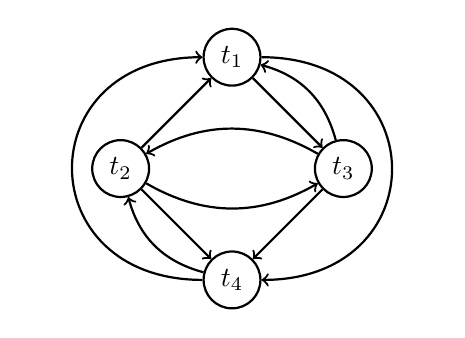
\begin{tikzpicture}[node distance={2cm}, thick, main/.style = {draw, circle}]
        \node[main] (1) {$t_1$};
        \node[main] (2) [below left of=1] {$t_2$};
        \node[main] (3) [below right of=1] {$t_3$};
        \node[main] (4) [below right of=2] {$t_4$};
        % \node[main] (5) [below right of=3] {$t_5$};

        \path[->] (1) edge node {} (3);
        \path[->] (1) edge [in=0, out=0,looseness=2] node {} (4);

        \path[->] (2) edge [bend right] node {} (3);
        \path[->] (2) edge node {} (4);
        \path[->] (2) edge node {} (1);

        \path[->] (3) edge node {} (4);
        \path[->] (3) edge [bend right] node {} (1);
        \path[->] (3) edge [bend right] node {} (2);
        % \path[->] (3) edge [out=50,in=120,looseness=2] node {} (2);

        \path[->] (4) edge [bend left] node {} (2);
        \path[->] (4) edge [in=180, out=180, looseness=2] node {} (1);
        
    \end{tikzpicture}
    \caption{Serial (Conflict) Graph for $s_2$}
    \label{fig:conflict_graph_q1}
\end{figure}

\section*{Problem 4.9}
In figure \ref{fig:deadlock_q2}, $t_1$ will acquire lock on $y$ and $t_2$ will acquire lock on $x$. As we can share locks in O2PL, $t_2$ will be able to acquire lock on $y$ and $t_1$ will be able to acquire lock on $x$. But while releasing locks, we need to preserve order of locks. Now, $t_1$ will be waiting to release lock on $x$ by $t_2$ and $t_2$ will be waiting to release lock on $y$ by $t_1$. Hence, there will be a deadlock.
\begin{figure}[h]
    \centering
    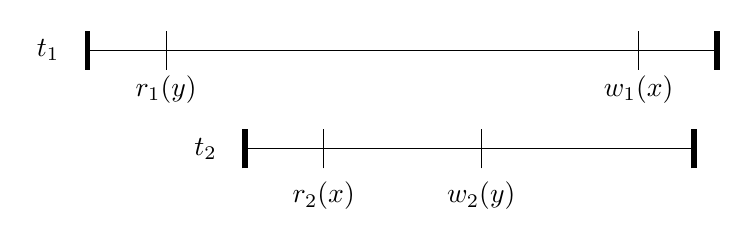
\begin{tikzpicture}
        \node at (-0.5, 0) {\(t_1\)};
        \draw[-] (0,0) -- (8, 0);
        \draw[line width=0.75mm] (0, -0.25) -- (0, 0.25);

        \draw[-] (1, -0.25) -- (1, 0.25);
        \node[below] at (1, -0.2)  {\(r_1(y)\)};
        
        \draw[-] (7, -0.25) -- (7, 0.25);
        \node[below] at (7, -0.2)  {\(w_1(x)\)};

        \draw[line width=0.75mm] (8, -0.25) -- (8, 0.25);

        \node at (1.5, -1.25) {\(t_2\)};
        \draw[-] (2, -1.25) -- (7.7, -1.25);
        \draw[line width=0.75mm] (2, -1.5) -- (2, -1);

        \draw[-] (3, -1.5) -- (3, -1.0);
        \node[below] at (3, -1.55)  {\(r_2(x)\)};

        \draw[-] (5, -1.5) -- (5, -1.0);
        \node[below] at (5, -1.55)  {\(w_2(y)\)};

        \draw[line width=0.75mm] (7.7, -1.5) -- (7.7, -1);
        
    \end{tikzpicture}
    \caption{O2PL deadlock}
    \label{fig:deadlock_q2}
\end{figure}

\section*{Problem 4.12}
The condition is semmingly natural but would lead to incorrect beahviour. If we remove a node, there is a possiblilty in future a cycle might be formed using the removed node, which will lead to incorrect behaviour of SGT protocol.
\begin{equation*}
    s = w_1(x) r_2(y) w_1(y) c_1 r_3(z) w_2(z) c_2 r_3(x) c_3
\end{equation*}

In figure \ref{fig:q3_1}, serialization graph is made using SGT protcol, and a cycle is formed. So, need to abort one of the transaction. \\
But if we use the given protocol in the question, we will remove $t_1$ after $c_2$ as $t_1$ is commited and active transaction at commit of $t_1$, i.e.,  $t_2$ is also commited. So, we will remove $t_1$ and the serialization graph will look like figure \ref{fig:q3_2}, which is acyclic (dashed line shows removed nodes). Hence suggested protocol is incorrect.

\begin{figure}[h]
    \centering
    
    % make two tikzpictures side by side
    \begin{minipage}{0.4\textwidth}
        \centering
        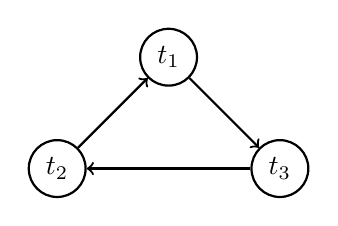
\begin{tikzpicture}[node distance={2cm}, thick, main/.style = {draw, circle}]
            \node[main] (1) {$t_1$};
            \node[main] (2) [below left of=1] {$t_2$};
            \node[main] (3) [below right of=1] {$t_3$};
            
            \path[->] (2) edge node {} (1);

            \path[->] (3) edge node {} (2);

            \path[->] (1) edge node {} (3);
        \end{tikzpicture}
        \caption{Without removing nodes}
        \label{fig:q3_1}
    \end{minipage}
    \begin{minipage}{0.4\textwidth}
        \centering
        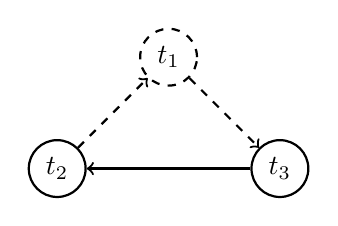
\begin{tikzpicture}[node distance={2cm}, thick, main/.style = {draw, circle}]
            \node[main, dashed] (1) {$t_1$};
            \node[main] (2) [below left of=1] {$t_2$};
            \node[main] (3) [below right of=1] {$t_3$};
            
            \path[->, dashed] (2) edge node {} (1);

            \path[->] (3) edge node {} (2);

            \path[->, dashed] (1) edge node {} (3);
        \end{tikzpicture}
        \caption{With removing nodes}
        \label{fig:q3_2}
    \end{minipage}
\end{figure}

\section*{Problem 4.16}
\begin{equation*}
    s = r_1(x) r_2(x) r_1(y) r_3(x) w_1(x) w_1(y) c_1 r_2(y) r_3(z) w_3(z) c_3 r_2(z) c_2
\end{equation*}
\subsection*{BOCC}
In this case, $t_2$ and $t_3$ will be aborted. 
\begin{itemize}
    \item $t_2$ abort: Here, val/write phase of $t_1$ is before $t_2$. $RS(t_2) \cap WS(t_1) \neq \phi$, as $t_2$ reads $x$ and $t_1$ writes $x$. So, $t_2$ will be aborted.
    \item $t_3$ abort: Here, val/write phase of $t_1$ is before $t_3$. $RS(t_3) \cap WS(t_1) \neq \phi$, as $t_3$ reads $x$ and $t_1$ writes $x$. So, $t_3$ will be aborted.
\end{itemize}
Final schedule will be:
\begin{equation*}
    s = r_1(x) r_2(x) r_1(y) r_3(x) w_1(x) w_1(y) c_1 r_2(y) r_3(z) a_3 r_2(z) a_2
\end{equation*}

\subsection*{FOCC}
In this case $t_1$ will be aborted.
\begin{itemize}
    \item $t_1$ abort: As $WS(t_1) \cap RS(t_2) \neq \phi$, as $t_1$ writes $x$ and $t_2$ reads $x$. Also, $WS(t_1) \cap RS(t_3) \neq \phi$, as $t_1$ writes $x$ and $t_3$ reads $x$. So, $t_1$ will be aborted.
\end{itemize}
Final schedule will be:
\begin{equation*}
    s = r_1(x) r_2(x) r_1(y) r_3(x) a_1 r_2(y) r_3(z) w_3(z) c_3 r_2(z) c_2
\end{equation*}

\end{document}